\documentclass[margin=10pt]{standalone} 
            \usepackage{color,xcolor} 
            \usepackage{tikz-qtree, tikz} 
            \usepackage[utf8]{inputenc} 
            \usetikzlibrary{decorations.pathreplacing,arrows,shapes,positioning,shadows,calc}
            \usetikzlibrary{decorations, decorations.text,backgrounds}
            \tikzset{every picture/.style={font issue=\footnotesize}, font issue/.style={execute at begin picture={#1\selectfont}}}
            
                    \begin{document}
                        \centering
                            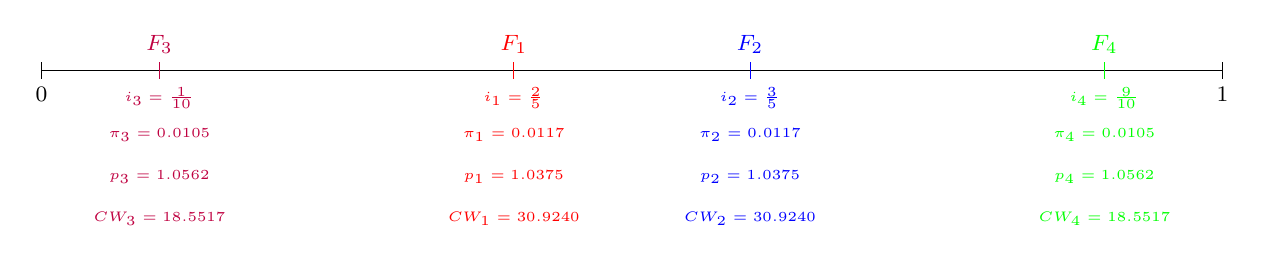
\begin{tikzpicture}

                            % Nodes 0 and 1
                            \draw (0,0) -- (15,0);
                            \draw (0 cm,3pt) -- (0 cm,-3pt);
                            \draw (15 cm,3pt) -- (15 cm,-3pt);
                % Firm0Choice
\draw [red] (2/5 * 15 cm,3pt) -- (2/5 * 15 cm,-3pt);
\draw (2/5 * 15 cm,0) node[above=3pt, red] {$ F_1$} node[above=3pt] {$ $};
\draw (2/5 * 15 cm,0) node[below=3pt, red] {\tiny $ i_1=\frac{2}{5}$} node[above=3pt] {$ $};
\draw (2/5 * 15 cm,0) node[below=18pt, red] {\tiny $ \pi_1=0.0117$} node[above=3pt] {$ $};
\draw (2/5 * 15 cm,0) node[below=33pt, red] {\tiny $ p_1=1.0375$} node[above=3pt] {$ $};
\draw (2/5 * 15 cm,0) node[below=48pt, red] {\tiny $ CW_1=30.9240$} node[above=3pt] {$ $};
% Firm1Choice
\draw [blue] (3/5 * 15 cm,3pt) -- (3/5 * 15 cm,-3pt);
\draw (3/5 * 15 cm,0) node[above=3pt, blue] {$ F_2$} node[above=3pt] {$ $};
\draw (3/5 * 15 cm,0) node[below=3pt, blue] {\tiny $ i_2=\frac{3}{5}$} node[above=3pt] {$ $};
\draw (3/5 * 15 cm,0) node[below=18pt, blue] {\tiny $ \pi_2=0.0117$} node[above=3pt] {$ $};
\draw (3/5 * 15 cm,0) node[below=33pt, blue] {\tiny $ p_2=1.0375$} node[above=3pt] {$ $};
\draw (3/5 * 15 cm,0) node[below=48pt, blue] {\tiny $ CW_2=30.9240$} node[above=3pt] {$ $};
% Firm2Choice
\draw [purple] (1/10 * 15 cm,3pt) -- (1/10 * 15 cm,-3pt);
\draw (1/10 * 15 cm,0) node[above=3pt, purple] {$ F_3$} node[above=3pt] {$ $};
\draw (1/10 * 15 cm,0) node[below=3pt, purple] {\tiny $ i_3=\frac{1}{10}$} node[above=3pt] {$ $};
\draw (1/10 * 15 cm,0) node[below=18pt, purple] {\tiny $ \pi_3=0.0105$} node[above=3pt] {$ $};
\draw (1/10 * 15 cm,0) node[below=33pt, purple] {\tiny $ p_3=1.0562$} node[above=3pt] {$ $};
\draw (1/10 * 15 cm,0) node[below=48pt, purple] {\tiny $ CW_3=18.5517$} node[above=3pt] {$ $};
% Firm3Choice
\draw [green] (9/10 * 15 cm,3pt) -- (9/10 * 15 cm,-3pt);
\draw (9/10 * 15 cm,0) node[above=3pt, green] {$ F_4$} node[above=3pt] {$ $};
\draw (9/10 * 15 cm,0) node[below=3pt, green] {\tiny $ i_4=\frac{9}{10}$} node[above=3pt] {$ $};
\draw (9/10 * 15 cm,0) node[below=18pt, green] {\tiny $ \pi_4=0.0105$} node[above=3pt] {$ $};
\draw (9/10 * 15 cm,0) node[below=33pt, green] {\tiny $ p_4=1.0562$} node[above=3pt] {$ $};
\draw (9/10 * 15 cm,0) node[below=48pt, green] {\tiny $ CW_4=18.5517$} node[above=3pt] {$ $};

                \draw (0,0) node[below=3pt] {$ 0 $} node[above=3pt] {$ $};
                
                \draw (15,0) node[below=3pt] {$ 1 $} node[above=3pt] {$ $};
                
            \end{tikzpicture}
            \end{document}
            